\section{Results}
To evaluate jump points we use a generic implementation of A* which we 
adapted to facilitate online neighbour pruning and jump point identification.
We discuss
performance in terms of \emph{speedup}: i.e. relative improvemement to the time 
taken to solve a given problem, and the number of nodes expanded, when searching
with and without graph pruning applied to the grid.
Using this metric a search time speedup
of 2.0 is twice as fast while a node expansion speedup of 2.0 indicates half the
number of nodes were expanded.  In each case higher is better.
Figure \ref{fig:speedup} shows average search time speedups across
each of our four benchmarks. Table \ref{table:nodes} shows average
node expansion speedups; the best results for each column are in bold.

\input table_nodes

\begin{figure*}[t]
   \begin{center}
	   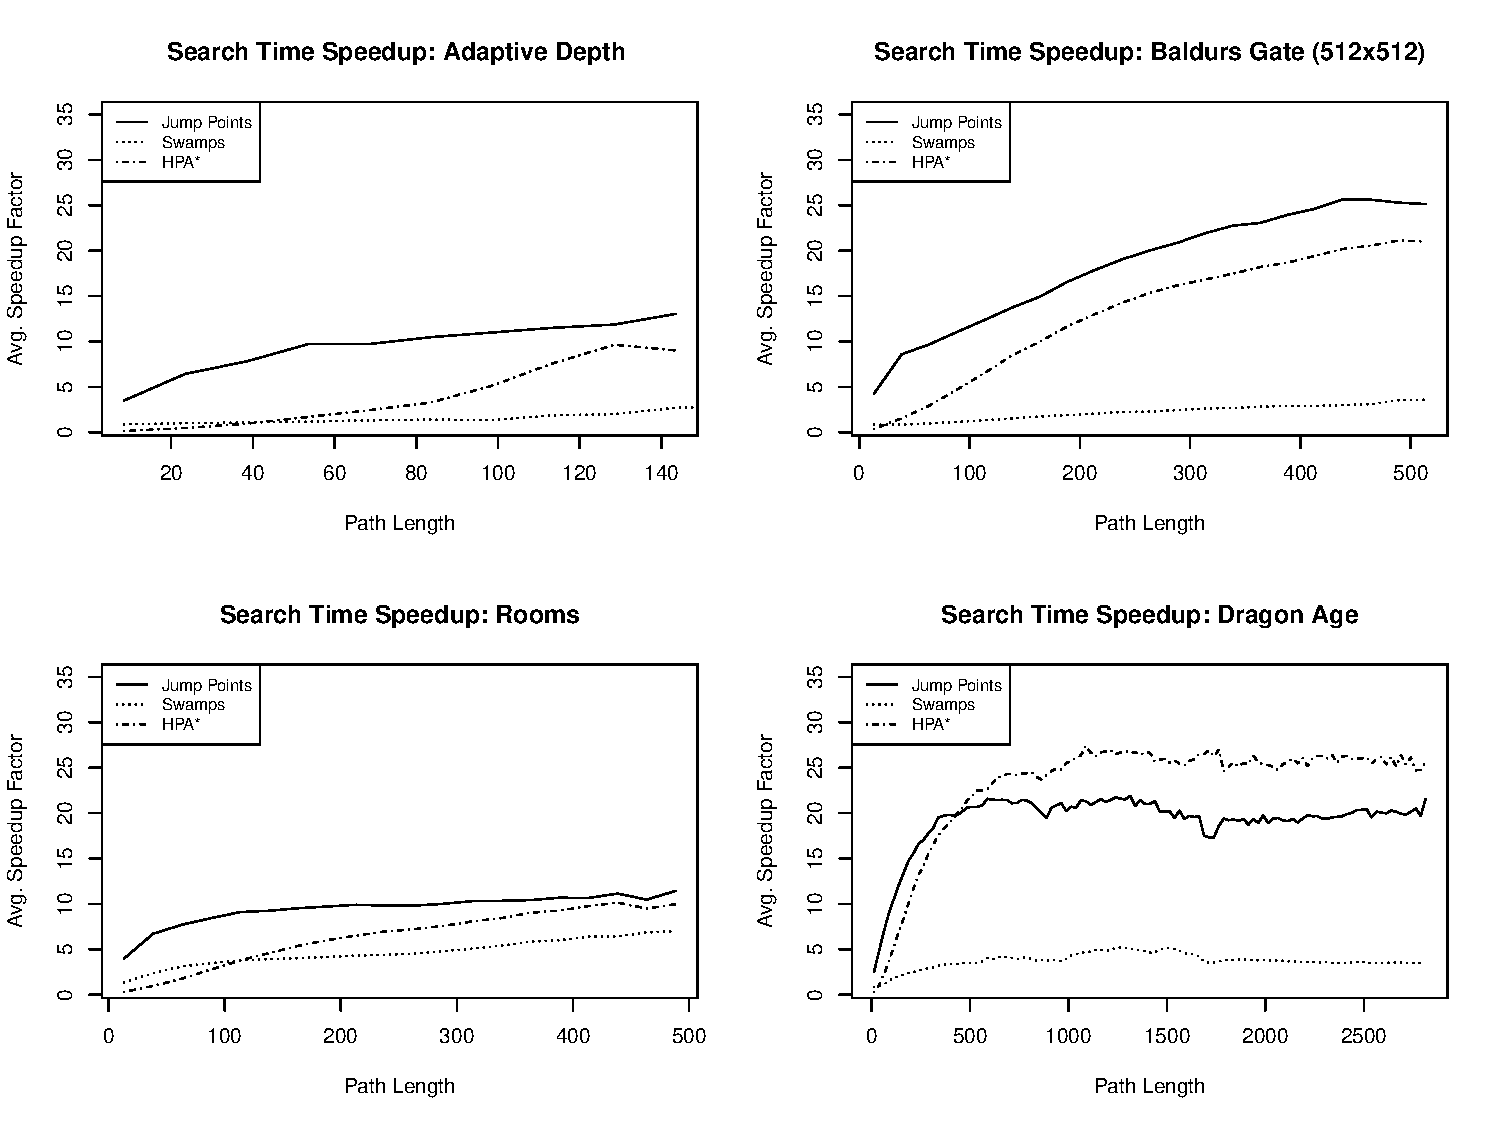
\includegraphics[width=2.0\columnwidth, trim = 10mm 10mm 10mm 0mm]
		{diagrams/speedup.pdf}
   \end{center}
   \caption{Average A* search time speedup on our each of our four benchmarks. }

\label{fig:speedup}
\end{figure*}

\textbf{Comparison with Swamps: }
We begin by comparing jump points to Swamps~\cite{pochter10}: an optimality
preserving pruning technique for speeding up pathfinding.  
We used the authors' source code, and their implementation of A*, and ran
all experiments using their recommended running parameters: a swamp seed radius
of 6 and ``no change limit'' of 2.

As per Figure \ref{fig:speedup}, jump point pruning shows a convincing
improvement to average search times across all benchmarks.
The largest differences are
observed on Baldur's Gate and Dragon Age where searching with jump points
reaches the goal 20-26 times sooner while searching with Swamps attains only a 3-5
times speedup.  Similar trends are observed when looking at Table
\ref{table:nodes}, where the improvement to the total number of nodes expanded
is even more pronounced.

Based on these results we conclude that while Swamps are effective for
identifying areas of the map not relevant to reaching the goal, those areas
which remain still require significant effort to search.  Jump points use a much
stronger yet orthogonal strategy to prove that many nodes expanded by Swamps can
be ignored.  As the two ideas appear complementary we posit that they could be
easily combined: first, apply a Swamps-based decomposition to prune areas not
relevant to the current search.  Then, use jump points to search the remaining
portions of the map.

\textbf{Comparison with HPA*: }
Next, we compare jump points pruning to the HPA* algorithm~\cite{botea04}.
Though sub-optimal, HPA* is very fast and widely applied in video games. We
compare against it to establish whether or not jump points are equally
applicable in similar contexts.  When evaluating HPA* we measure the total cost
of insertion and hierarchical search. We did not perform any path refinement 
nor path smoothing.
We configured HPA* with a single-level abstraction hierarchy and a
fixed cluster size of 10.  These settings are recommended by the original
authors who note that larger cluster sizes and more levels can often incur
significant overhead.

As per Figure \ref{fig:speedup}, jump points pruning is shown to be 
highly competitive with HPA*.
On Adaptive Depth, Baldur's Gate and Rooms, jump points have a clear advantage
-- improving on HPA* search times by several factors in some cases.
On the Dragon Age benchmark jump points have a small advantage for problems of 
length $< 500$ but for longer instances there is very little between the two
algorithms.
Table \ref{table:nodes} provides further insight: although searching with jump 
points expands significantly fewer nodes than HPA*, each such operation
takes longer.

We conclude that jump point pruning is a competitive substitute for HPA* and,
for a wide variety of problems, can help to find solutions significantly faster.
HPA*
can still be advantageous, particularly if a small memory overhead is acceptable
and optimality is not important, but only if the cost of inserting the start and
goal nodes into the abstract graph, and the cost of the subsequent refinement
phase, can be sufficiently amortized over the time required to find an abstract
path.
One direction for further work could be to use jump
point pruning to speed up HPA*: for example during insertion and refinement.
